\documentclass[12pt,letterpaper]{article}
\usepackage[utf8]{inputenc}
\usepackage[spanish]{babel}
\usepackage{graphicx}
\usepackage[left=2cm,right=2cm,top=2cm,bottom=2cm]{geometry}
\usepackage{graphicx} % figuras
% \usepackage{subfigure} % subfiguras
\usepackage{float} % para usar [H]
\usepackage{amsmath}
%\usepackage{txfonts}
\usepackage{stackrel} 
\usepackage{multirow}
\usepackage{enumerate} % enumerados
\renewcommand{\labelitemi}{$-$}
\renewcommand{\labelitemii}{$\cdot$}
% \author{}
% \title{Caratula}
\begin{document}

% Fancy Header and Footer
% \usepackage{fancyhdr}
% \pagestyle{fancy}
% \cfoot{}
% \rfoot{\thepage}
%

% \usepackage[hidelinks]{hyperref} % CREA HYPERVINCULOS EN INDICE

% \author{}
\title{Caratula}

\begin{titlepage}
\begin{center}
\large{UNIVERSIDAD PRIVADA-DE-TACNA}\\
\vspace*{-0.025in}
\begin{figure}[htb]
\begin{center}

\end{center}
\end{figure}
\begin{center}
    
\includegraphics[width=5cm, height=5cm]{img/upt.jpg}  
\end{center}

\vspace*{0.15in}
INGENIERIA DE SISTEMAS  \\

\vspace*{0.5in}
\begin{large}
TITULO:\\
\end{large}

\vspace*{0.1in}
\begin{Large}
\textbf{Laboratorio N° 01 Creando una base de datos Clave-Valor} \\
\end{Large}

\vspace*{0.3in}
\begin{Large}
\textbf{CURSO:} \\
\end{Large}

\vspace*{0.1in}
\begin{large}
BASE DE DATOS II\\
\end{large}

\vspace*{0.3in}
\begin{Large}
\textbf{DOCENTE:} \\
\end{Large}

\vspace*{0.1in}
\begin{large}
Ing. Patrick Cuadros Quiroga\\
\end{large}

\vspace*{0.2in}
\vspace*{0.1in}
\begin{large}
Alumno: \\
\begin{flushleft}
 Herrera Amezquita, Derian Francisco		\hfill	(2017059489) \\


\end{flushleft}
\end{large}
\end{center}

\end{titlepage}



\tableofcontents % INDICE
\thispagestyle{empty} % INDICE SIN NUMERO
\newpage
\setcounter{page}{1} % REINICIAR CONTADOR DE PAGINAS DESPUES DEL INDICE


Abra la consola de administración de AWS para poder mantener abierta esta guía paso a paso. Cuando se cargue esta pantalla empiece a escribir DynamoDB en la barra de búsqueda y seleccione la opción para abrir la consola de DynamoDB.

\begin{center}
    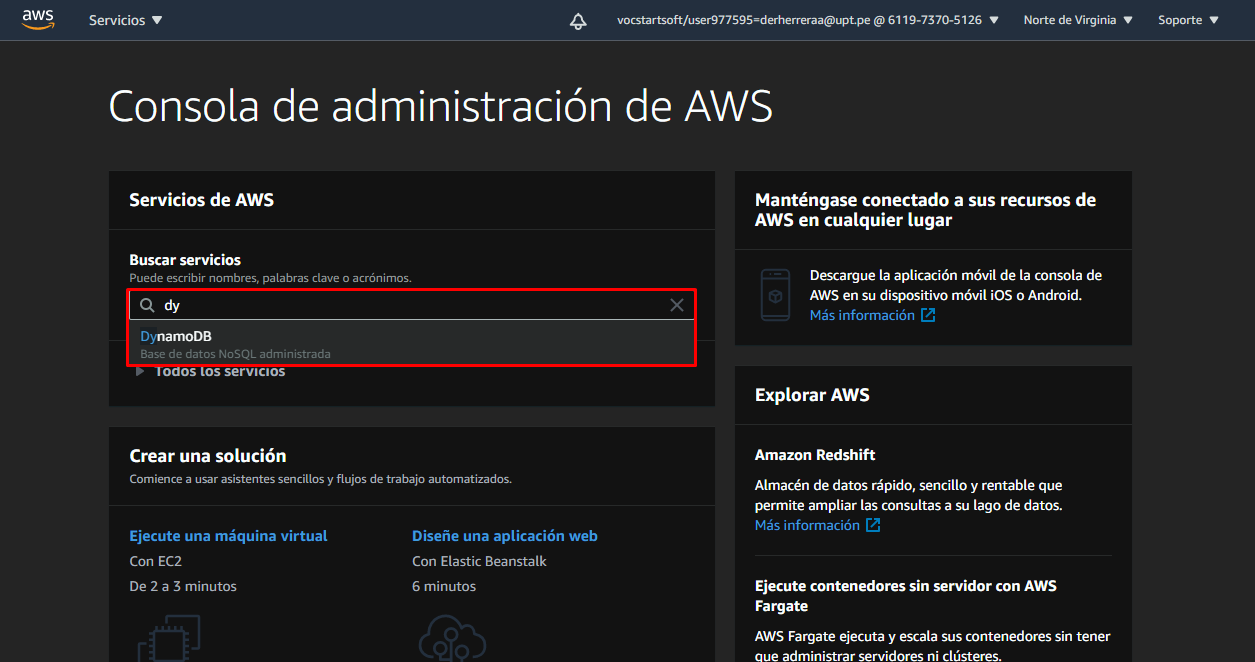
\includegraphics[width=18cm, height=10cm]{img/1.png}  
\end{center}
\newpage
\section{Paso 1: creación de una tabla NoSQL
} 

a. En la consola de DynamoDB, haga clic en Create table (Crear tabla).
\begin{center}
    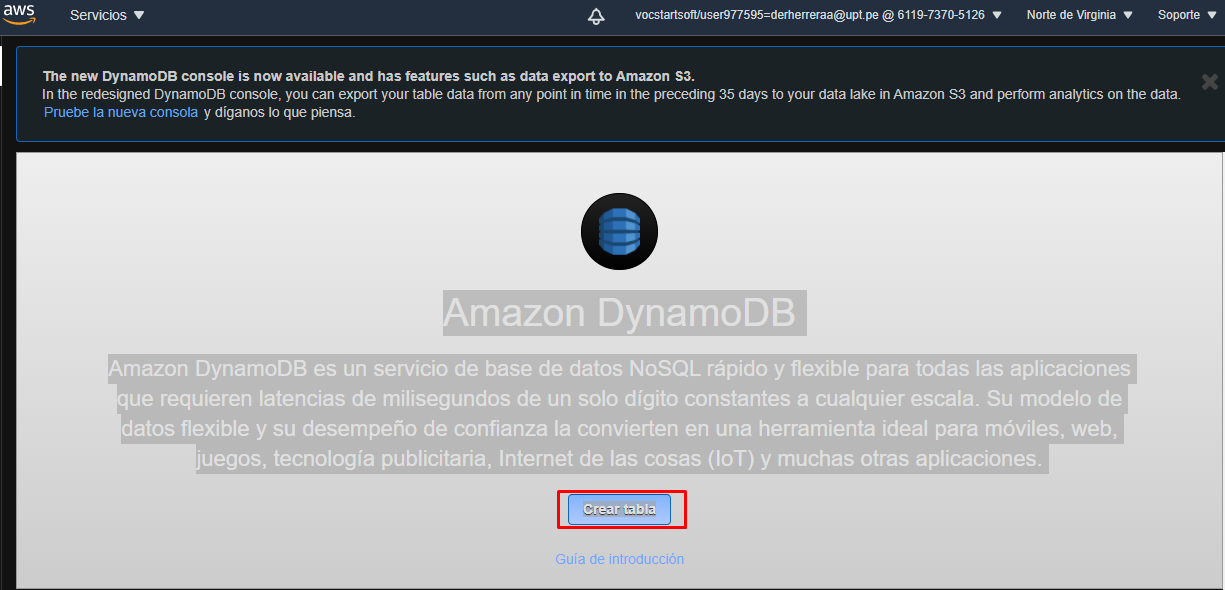
\includegraphics[width=18cm, height=10cm]{img/2.png}  
\end{center}

b. En el campo Table name (Nombre de la tabla), escriba Music.

\begin{center}
    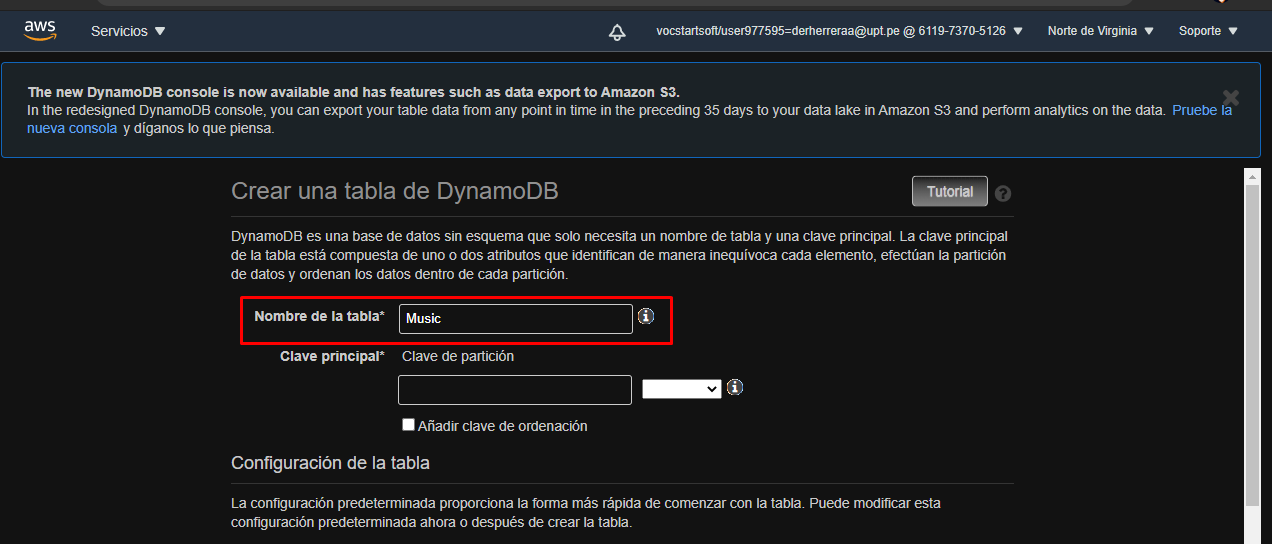
\includegraphics[width=18cm, height=10cm]{img/3.png}  
\end{center}


c. Escriba Artist en el campo Partition Key (Clave de partición).
\begin{center}
    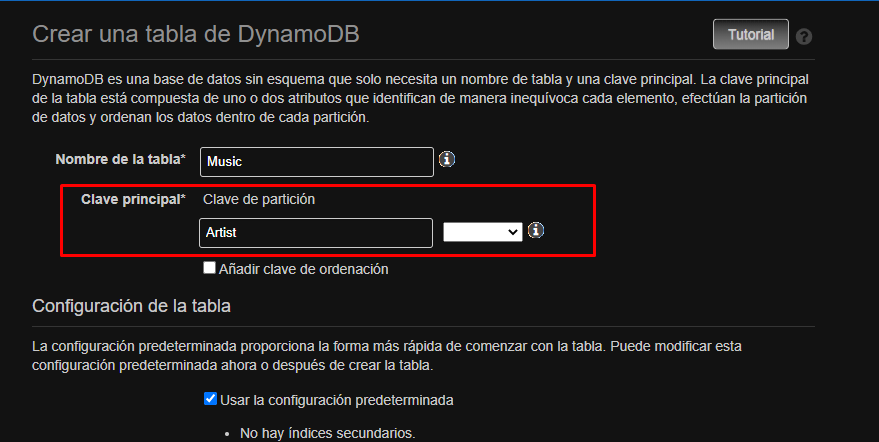
\includegraphics[width=18cm, height=10cm]{img/4.png}  
\end{center}

d. Dado que cada artista puede componer muchas canciones, puede habilitar el ordenamiento sencillo con una clave de ordenamiento. Marque la casilla Add sort key (Añadir clave de ordenamiento). Escriba songTitle en el campo Add sort key (Añadir clave de ordenamiento).
\begin{center}
    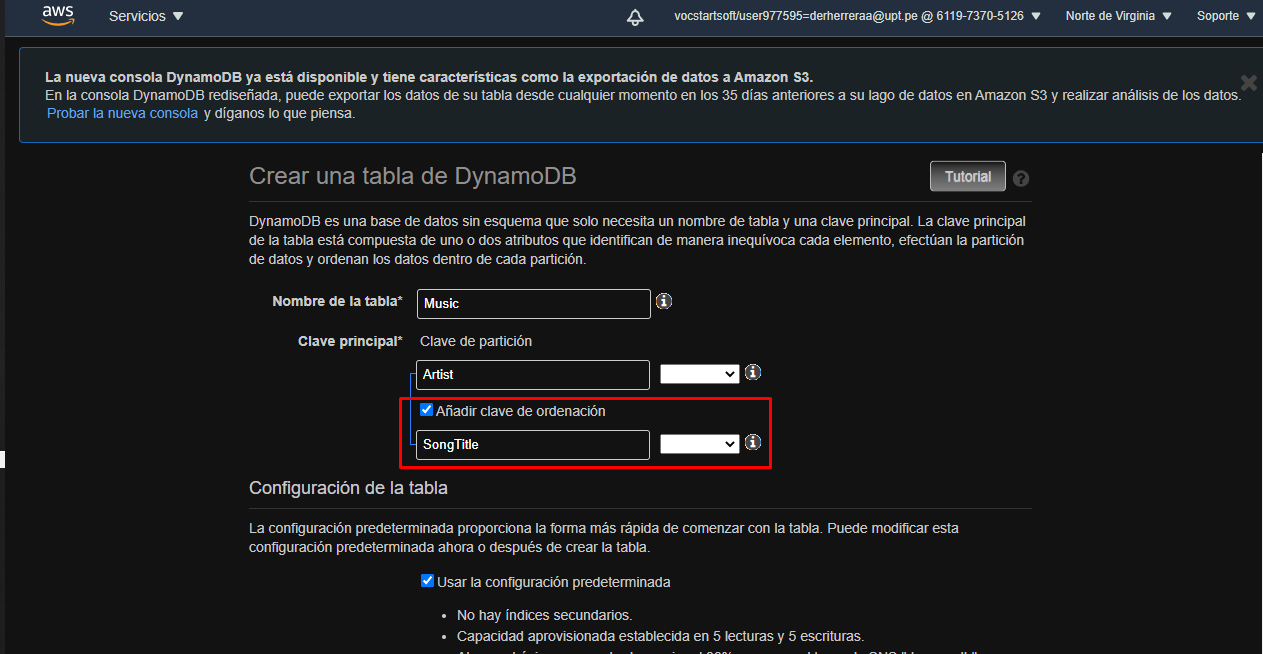
\includegraphics[width=18cm, height=10cm]{img/d.png}  
\end{center}

e. A continuación, activaremos DynamoDB Auto Scaling para nuestra tabla.
\begin{center}
    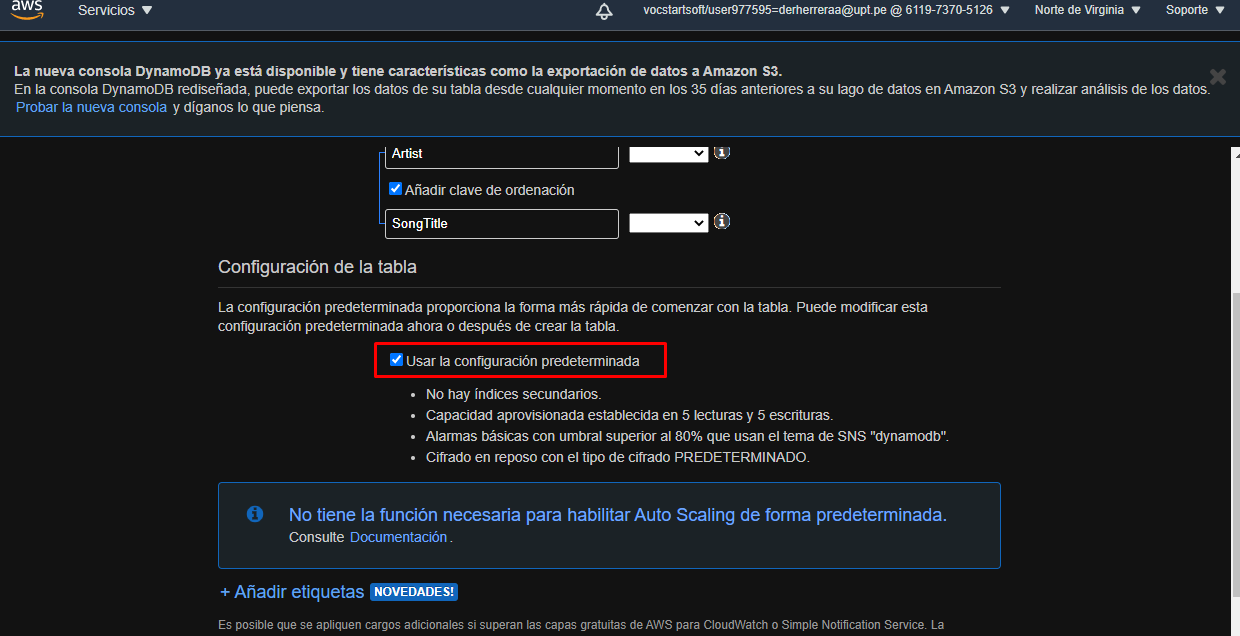
\includegraphics[width=18cm, height=10cm]{img/e.png}  
\end{center}

f. Desplácese hacia la parte inferior de la pantalla, pasando Secondary indexes (Índices secundarios), Provisioned capacity (Capacidad aprovisionada) y Auto Scaling hasta llegar al botón Create (Crear). 

\begin{center}
    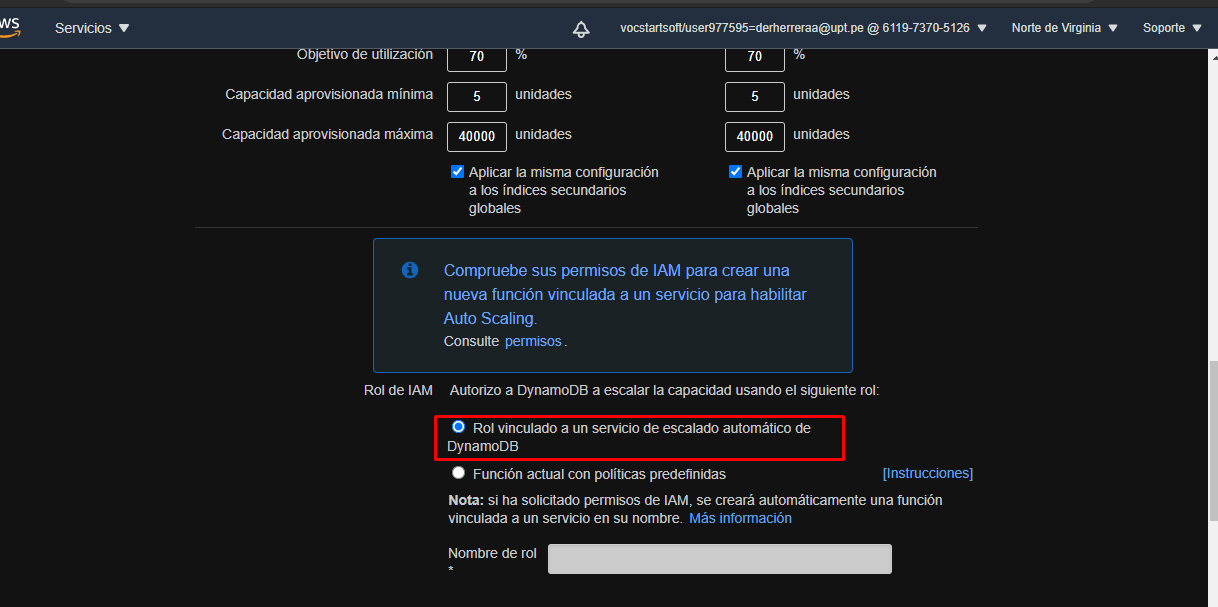
\includegraphics[width=18cm, height=10cm]{img/f.png}  
\end{center}
\begin{center}
    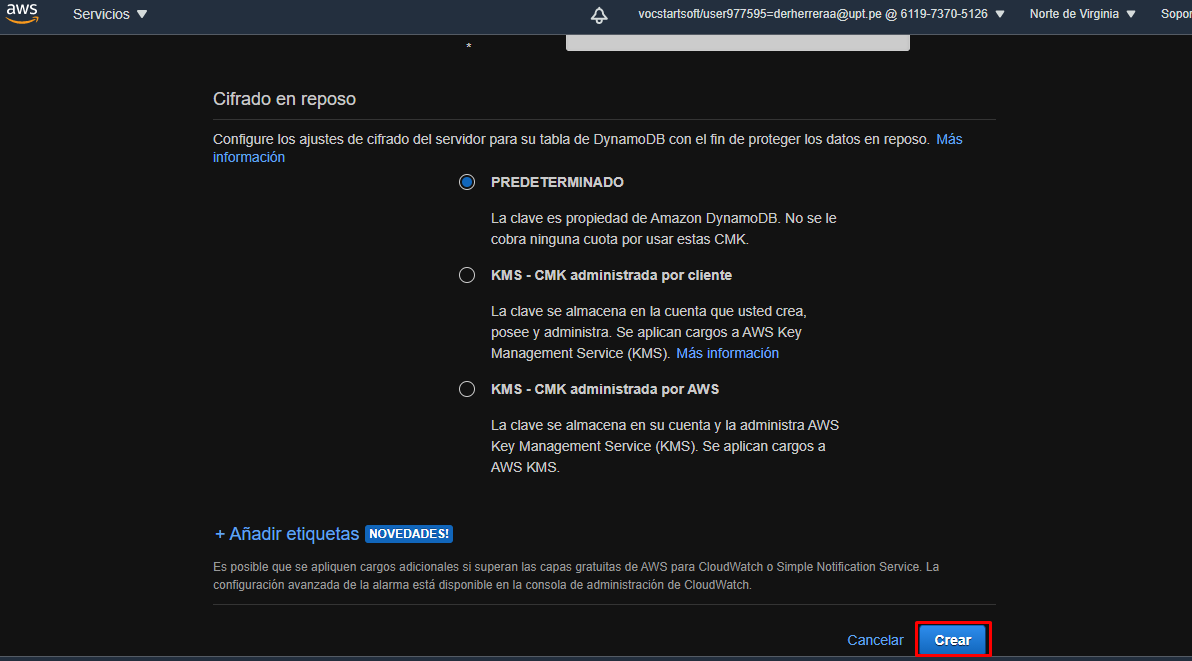
\includegraphics[width=18cm, height=10cm]{img/f.2.png}  
\end{center}
\newpage
\section{Paso 2: agregar datos a la tabla NoSQL
} 

a. Haga clic en la pestaña Items (Elementos). Bajo la pestaña Items (Elementos), haga clic en Create item (Crear elemento) .
\begin{center}
    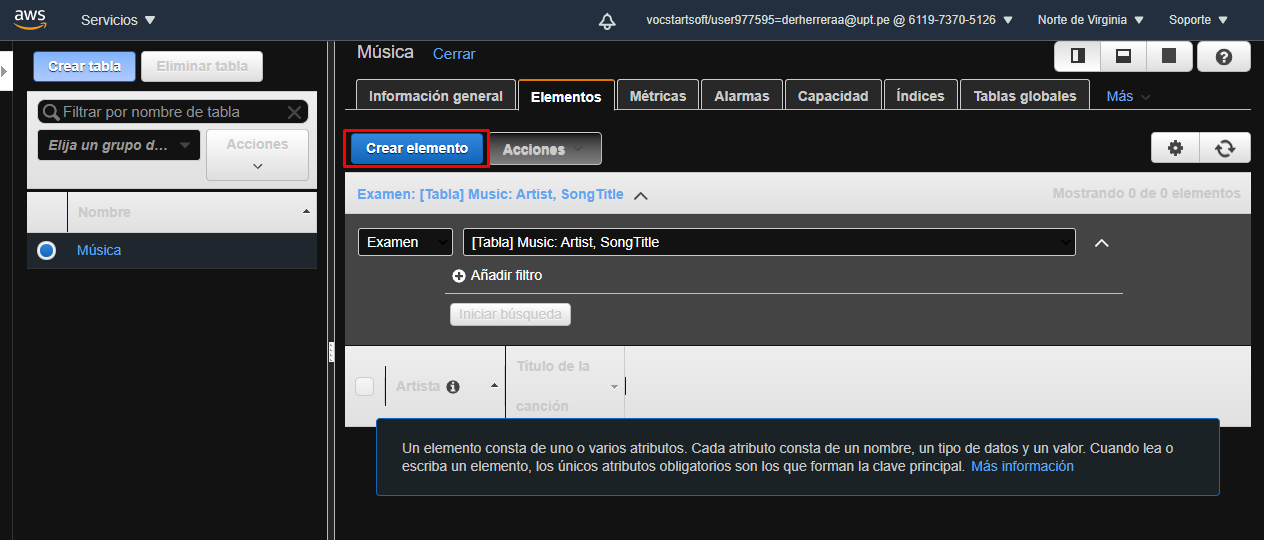
\includegraphics[width=18cm, height=7cm]{img/2a.png}  
\end{center}


b. En la ventana de introducción de datos, escriba lo siguiente:

Para el atributo Artist, escriba No One You Know.
\\Para el atributo SongTitle , escriba Call Me Today.
\\Haga clic en Save (Guardar) para guardar el elemento.
\begin{center}
    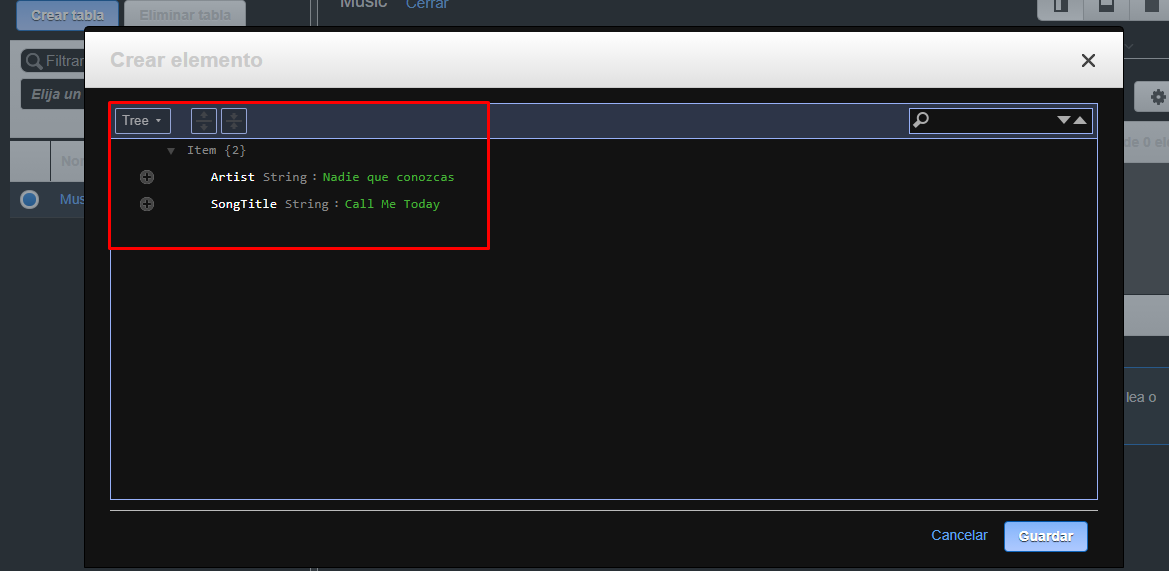
\includegraphics[width=18cm, height=8cm]{img/2b.png}  
\end{center}

\newpage
c. Repita el proceso para agregar algunos elementos más a la tabla Music:

Artist: No One You Know; songTitle: My Dog Spot
\\Artist: No One You Know; songTitle: Somewhere Down The Road
\\Artist: The Acme Band; songTitle: Still in Love
\\Artist: The Acme Band; songTitle: Look Out, World
\begin{center}
    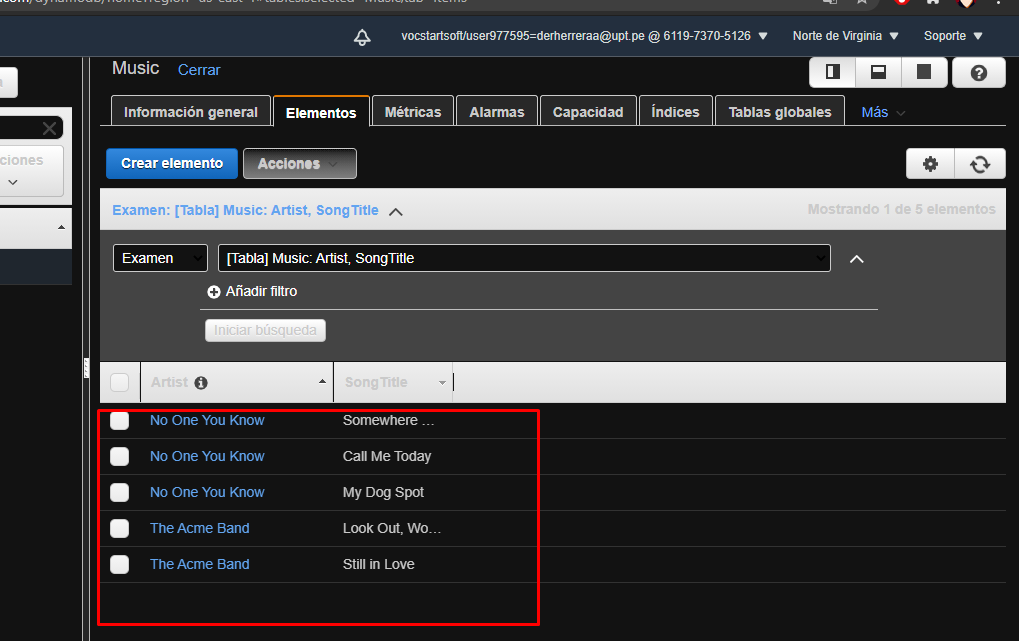
\includegraphics[width=18cm, height=7cm]{img/2c.png}  
\end{center}

\newpage

\section{Paso 3: consulta de la tabla NoSQL
} 
Las operaciones de consulta de DynamoDB son eficientes y utilizan claves para encontrar datos. Las operaciones de escaneo atraviesan la tabla entera.


a. Mediante la lista desplegable situada en el banner gris oscuro encima de los elementos, cambie Scan (Escaneo) a Query (Consulta). 

\begin{center}
    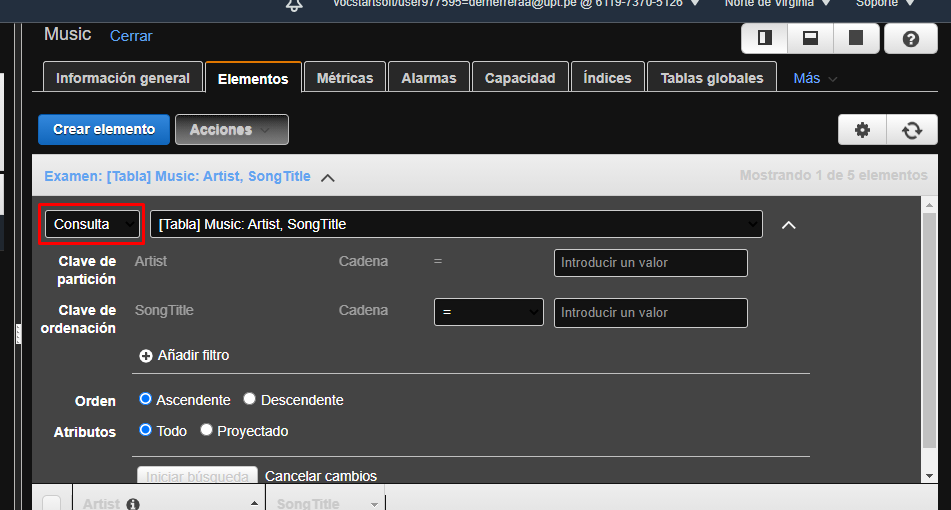
\includegraphics[width=18cm, height=10cm]{img/3a.png}  
\end{center}


\newpage
b. Puede utilizar la consola para consultar la tabla Music de diversas formas. Para la primera consulta, realice lo siguiente:

En el campo Artist, escriba No One You Know y luego haga clic en Start search (Iniciar búsqueda). Se muestran todas las canciones interpretadas por No One You Know.


\begin{center}
    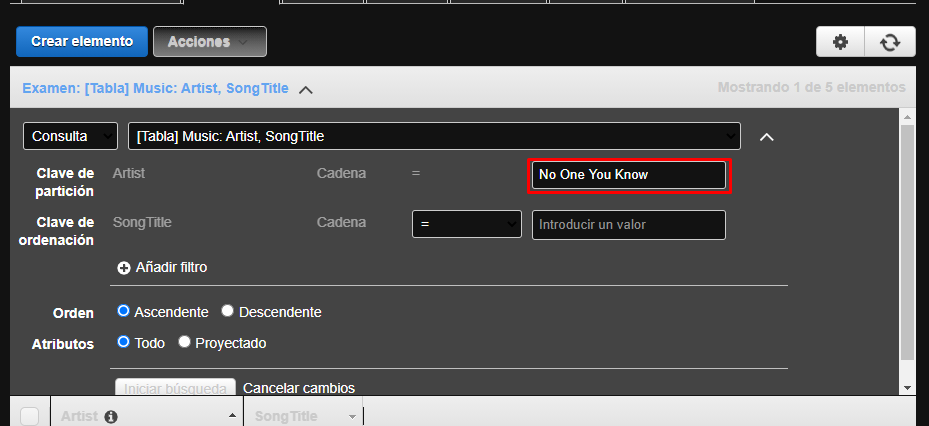
\includegraphics[width=18cm, height=7cm]{img/3b.png}  
\end{center}

c. Pruebe con otra consulta, pero esta vez acote los resultados de búsqueda:

En el campo Artist, escriba The Acme Band.
\\En el campo SongTitle, seleccione Begins with (Empieza por) en la lista desplegable y escriba S.
\\Haga clic en Start search (Iniciar búsqueda).  Solo se muestra “Still in Love” interpretada por The Acme Band.
\begin{center}
    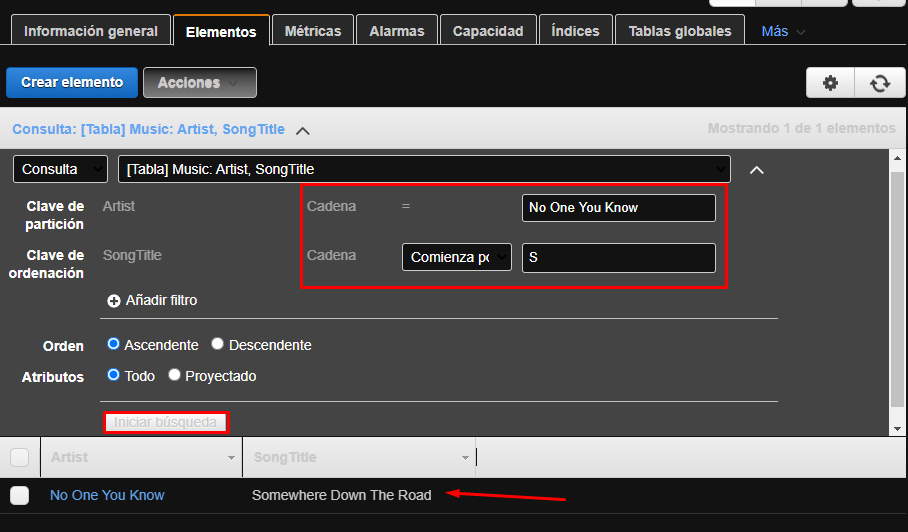
\includegraphics[width=18cm, height=10cm]{img/3C.png}  
\end{center}
\section{Paso 4: eliminación de un elemento existente
} 

En este paso, eliminará un elemento de la tabla de DynamoDB.

a. Seleccione el desplegable Query (Consulta) para que vuelva a aparecer Scan (Escaneo).  

Haga clic en la marca de verificación situada junto a The Acme Band. En el desplegable Actions (Acciones), seleccione Delete (Eliminar). Se le preguntará si desea eliminar el elemento. Haga clic en Delete (Eliminar) y se eliminará el elemento.
\begin{center}
    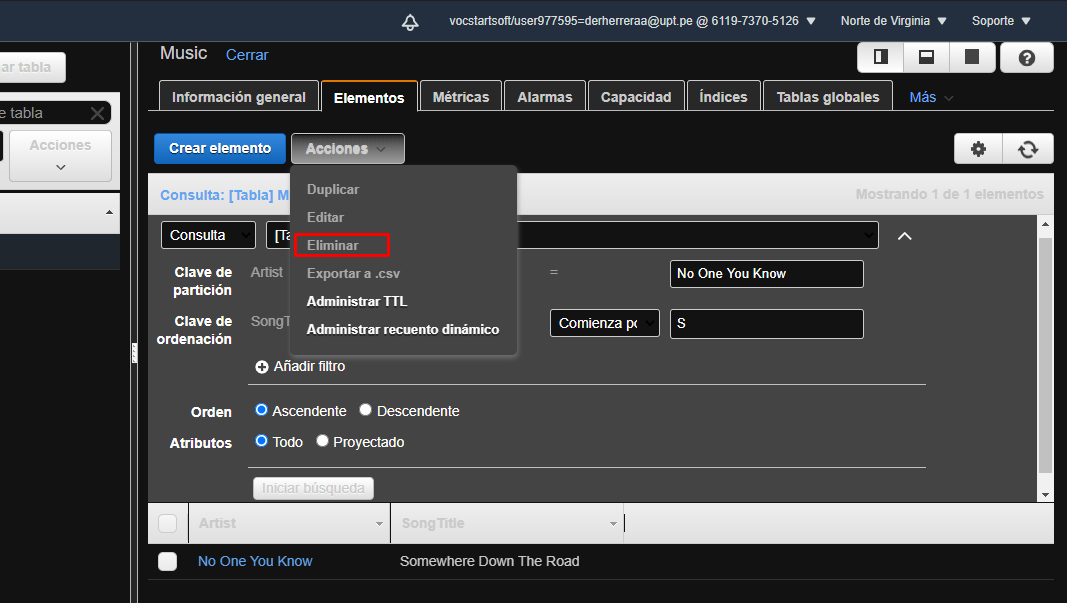
\includegraphics[width=18cm, height=10cm]{img/4A.png}  
\end{center}
\newpage
\section{Paso 5: eliminación de una tabla NoSQL
} 

En este paso, eliminará la tabla de DynamoDB.

a. Puede eliminar con facilidad una tabla de la consola Amazon DynamoDB. Se recomienda eliminar las tablas que ya no utilice para que no le sigan cobrando por ellas.

En la consola de DynamoDB, haga clic en el botón de selección ubicado junto a la tabla Music y, a continuación, haga clic en Delete table (Eliminar tabla).
\\En el cuadro de diálogo de confirmación, haga clic en Delete (Eliminar).

\begin{center}
    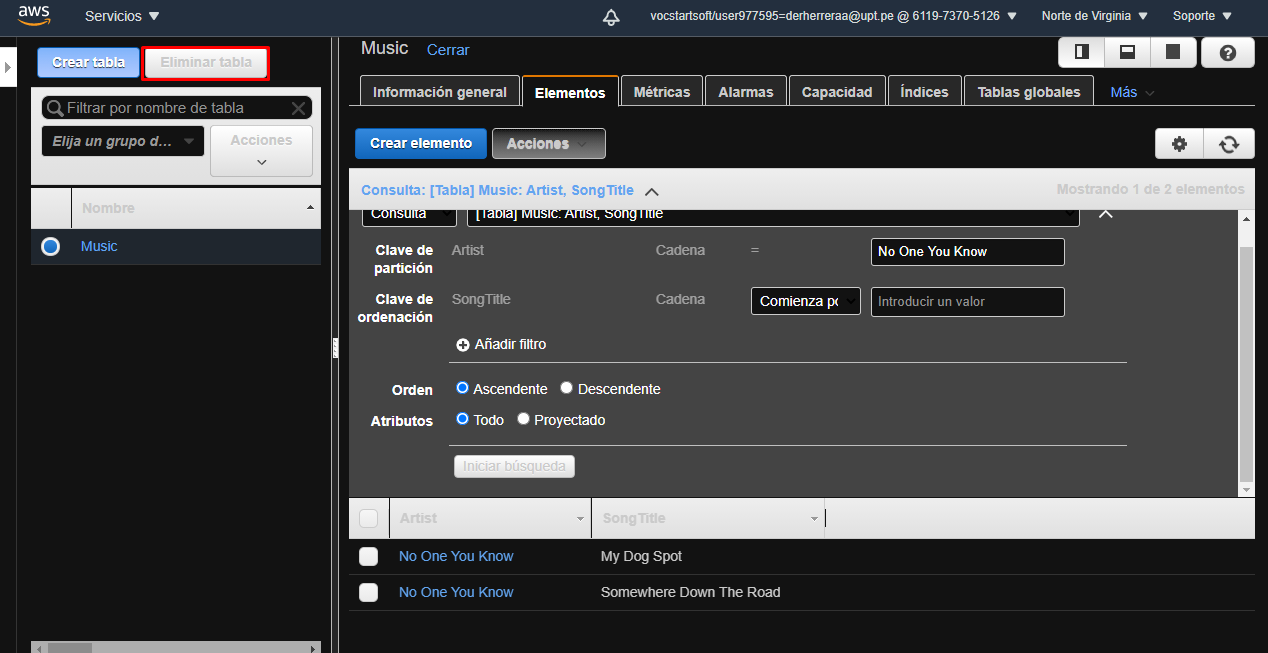
\includegraphics[width=18cm, height=8cm]{img/ELIMINAR.png}  
\end{center}

\begin{center}
    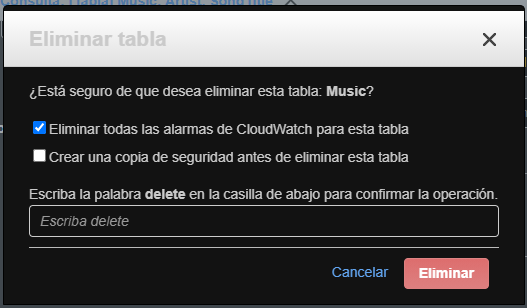
\includegraphics[width=18cm, height=8cm]{img/ELIMINAR2.png}  
\end{center}
\begin{center}
    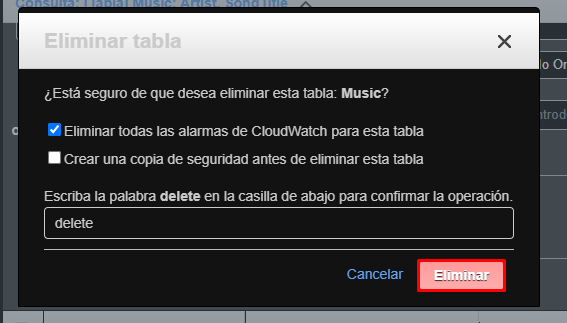
\includegraphics[width=18cm, height=10cm]{img/eliminar3.png}  
\end{center}
\begin{center}
    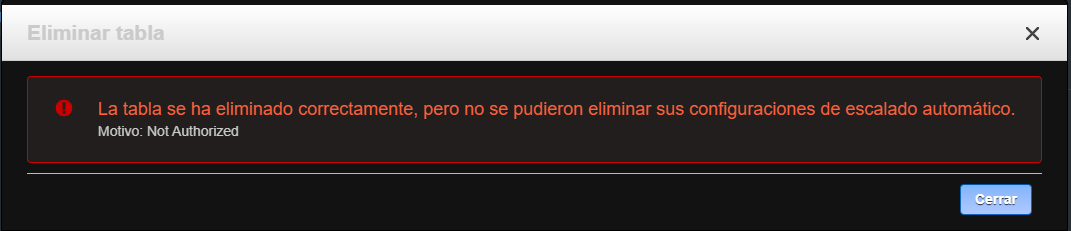
\includegraphics[width=18cm, height=3cm]{img/eliminar4.png}  
\end{center}





















\end{document}
